%!TEX root = _thesis.tex
\chapter{手指使用量常時計測の理論と計測ステム構築}

\section{ハンドジェスチャーインターフェース}
ハンドジェスチャーインターフェースの開発は,主にData glove型とMotion Capture System型の二つがベースとなっている.
Data glove型は各指の関節の曲がりの正確な測定するために,いくつかのフレックスセンサーを組み込んでいるが,これらは使用時にユーザが折り曲げる必要があり,スムーズな手指の動きを阻害していまう.また,正確な関節角度の測定に使われるフレックスセンサーは一般的に高価である.
一方,ビジョンベースのMotion Capture System型アプローチでは,ユーザーは特別な機器を着用する必要がない.
ただし,固定カメラを使用したビデオベースのMotion Capture Systemでは,一般に指のトラッキングが正確ではなく,ユーザーの手の動きがカメラの視野に制限される.
また,カメラを利用したシステムは高価であり,常にユーザの手指運動を測定するためにはユーザの腕に重さのあるカメラを装着する必要がある.
そのため,日常生活上での麻痺肢の使用量を測定することに向かない.

\section{手指使用量の常時計測方法}
既存の手法の問題点を考察すると,手指使用量の常時計測に向いた計測手法は以下の要件を満たす必要がある.

\begin{itemize}
 \item 計測機器が持ち運びやすい
 \item ノイズに対してロバストである
 \item 定量的である
 \item キャリブレーションが簡単でユーザへの負担が少ない
 \item 安価である
 \item 精度の高い指の関節角度測定ができる
\end{itemize}

そのため,これらの要件を満たし,手指使用量が計測可能なウェアラブルデバイスの開発を目的とする.計測機器を持ち運びやすくするには軽量でコンパクトな設計が求められる.

\section{指の関節角度計測}
本研究の手指使用量の測定手法は,指の関節角度の変化が,指の使用量を反映するという仮定に基づく.これは,指の関節角度が変化している場合,指が動いており,指を使っていると考えられるためである.

関節角度の変化の推定には,ウェアラブルデバイスに搭載された赤外線距離センサを用いる.本デバイスは指の基節に装着して使用し,赤外線距離センサで,デバイスから中節までの距離を常時計測する.式\ref{eq:theta}の関数を用い,測定された距離を指の関節角度に変換し,指の使用量を測る.距離を角度変換する模式図をFig.\ref{fig:principle}に示す.

\begin{figure}[H]
  \centering
  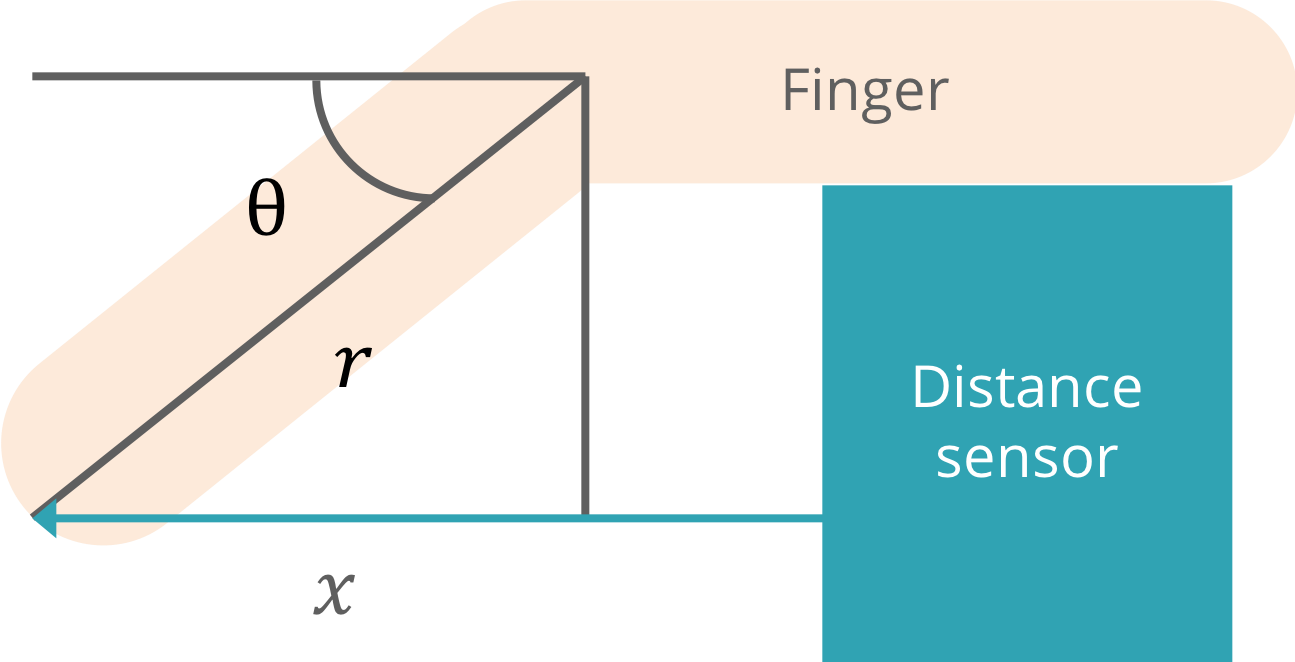
\includegraphics[width=0.8\linewidth]{fig/principle}
  \caption{Measurement principle}
  \label{fig:principle}
\end{figure}
Fig.\ref{fig:principle}のパラメータの関係を以下の式に表す.

\begin{equation}
\cos\theta = \frac{x}{r} 
\end{equation}
より
\begin{equation}
\theta = \cos^{-1} \frac{x}{r}
\label{eq:theta}
\end{equation}
である.

ここで,$r$は第二関節から指先までの長さ,$x$は最大屈曲時からの変化距離,$\theta$は最大伸展時からの変化角度である.
$r$は定数であり,デバイス使用前に物差しやスケール等を用い測定しておく必要がある.
$x$は本デバイスの赤外線距離センサによって推定する.$x$の推定方法は後述する.
この$r,x$の二つのパラメータと式\ref{eq:theta}を用いることで,関節角度$\theta$を推定する.

\section{ウェアラブルデバイスのハードウェア}
本デバイスは加速度計と赤外線距離センサの2つのセンシング部と,センシングされたデータを格納するデータ記録部からなるウェアラブルデバイスである.
本研究で開発したウェアラブルデバイスをFig.\ref{fig:device}に示す.
\begin{figure}[H]
  \centering
  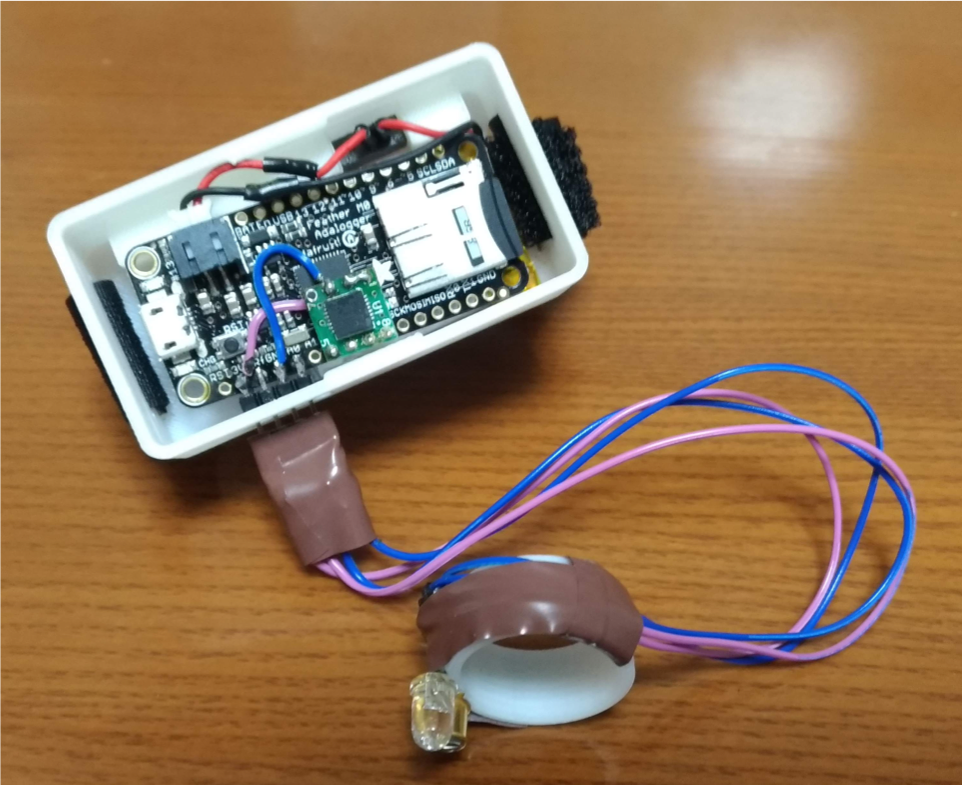
\includegraphics[width=0.8\linewidth]{fig/fal6}
  \caption{Hardware of the wearable device}
  \label{fig:device}
\end{figure}
ハードウェアとしては,赤外線距離センサが取り付けられた指輪部と,加速度センサが搭載されたマイクロコンピュータで成る腕輪部に分かれている.
デバイスの重さは,指輪部が5g(ワイヤ含む),腕輪部は30gである.
また,デバイスの大きさは,指輪部が直径20mm,厚さ2mm,長さ10mmである.腕輪部は63mm,34mm,20mmである.
本デバイスの指輪型の装着部分及び,バッテリーとマイコン基盤を収納するためのケースを3DCAD(Fusion 360)で設計し,3Dプリンタ(Dimension 1200es)で印刷し作成した.


\subsection*{センシング部}
距離計測と加速度計測を行うため,赤外線距離センサと加速度計の二つのセンサを利用した.
\subsubsection*{赤外線距離センサ}
指関節角度の変化をセンシングするため赤外線距離センサを使用した.
赤外線距離センサは発光ダイオード(Osram SFH4550)とフォトトランジスタセンサ(Honeywell SD5410)で構成されている.
赤外線距離センサは発光ダイオードが発光した際に出た光をフォトトランジスタで受光することで,距離を計測するセンサである.
フォトトランジスタの受光量は,ランベルトの反射の性質を有し,光が反射物に反射し受光素子に当たるまでの距離と角度,反射物の反射率により決定される(逆自乗の法則).そのため,センシングキャリブレーションを行った.センシングキャリブレーションに関しては後述する.
外部から入る光によるノイズを抑えるため,発光ダイオードとフォトトランジスタはそれぞれ6$^\circ$と12$^\circ$の狭い視覚野を持つパーツを選定した.手指の関節角度を測定するため,赤外線距離センサを指に取り付ける必要がある.
しかし,直接,テープや手袋などで赤外線距離センサを,ユーザの指に取り付けると,デバイスの装着や取り外しが煩雑になり,
ユーザへの負担が大きくなる問題が生じる.そのため,指輪型のハードウェアへ赤外線距離センサを取り付けた.これにより,ユーザにかかるデバイスの着脱による負荷を低減した.指輪型のハードウェアは3DCADで設計後,3Dプリンタを用いて作成した.

指輪型ハードウェアの大きさが,ユーザの指の太さと合っていない場合,センサのずれやユーザビリティの低下等の問題が発生する.
ユーザごとに指の太さが異なることが予想されるため,指輪の直径が異なる複数の指輪型のハードウェアを作成した.
日本人の平均的な食指の直径は,男性の場合19.6mm,SD=1.1,女性の場合17.5,SD=0.8である[65].
そのため17,18,19,20,21mmの直径を持つ指輪型ハードウェアを作成した.

\begin{figure}[H]
  \centering
  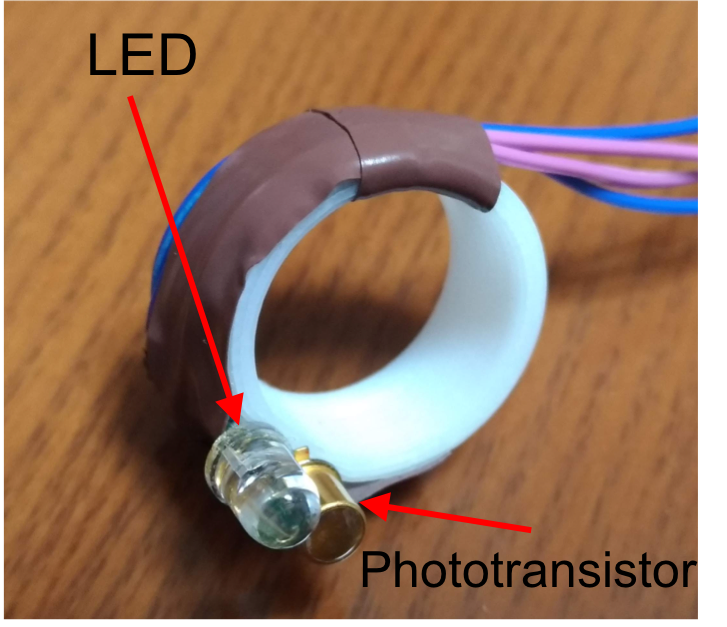
\includegraphics[width=0.8\linewidth]{fig/ring_led}
  \caption{Infrared distance sensor consists of LED and Phototransistor}
  \label{fig:distance sensor}
\end{figure}

赤外線距離センサはマイクロコンピュータとワイヤーで接続されており,マイクロコンピュータから給電を行なっている.また,フォトトランジスタがセンシングしたデータをマイクロコンピュータへ出力している.以下のFig.\ref{fig:circuit}に,赤外線距離センサとマイクロコンピュータ(Arduino)の接続を示す.
フォトトランジスタのサンプリング解像度は10bitのアナログ値であり100Hzのサンプリングレートでセンサ値を取得する.

\subsubsection*{三軸加速度センサ}
マイコン基盤に三軸加速度センサ(Kinonix KXR94-2050)を追加した.三軸加速度センサはAccelerometryと同様に,ユーザの腕の加速度を取得するために使用する.本実験で行うタスクは日常生活動作を踏襲したものとなっており,三次元の腕の動きが予想されるため,三軸の加速度センサを選定した.また,ウェアラブルデバイスに搭載するため,小型のセンサを選んだ.三軸加速度センサのスペックを以下に示す.

\begin{table}[H]
  \caption{Kinonix KXR94-2050の仕様}
  \centering
  \begin{tabular}{ll} 
    \hline \hline
測定レンジ&$\pm$ 2G\\
感度&660mV/g\\
測定出力&3軸アナログ出力(X,Y,Z)\\
非直線性誤差&0.1\%FS\\
出力帯域幅&800Hz\\
定格電源電圧&3.3V\\
動作電圧範囲&2.5$\sim$5.25V\\
    \hline
  \end{tabular}
\end{table}

三軸加速度センサの設置位置と,X,Y,Zの各軸をFig.\ref{fig:accelerometer}に示す.

\begin{figure}[H]
  \centering
  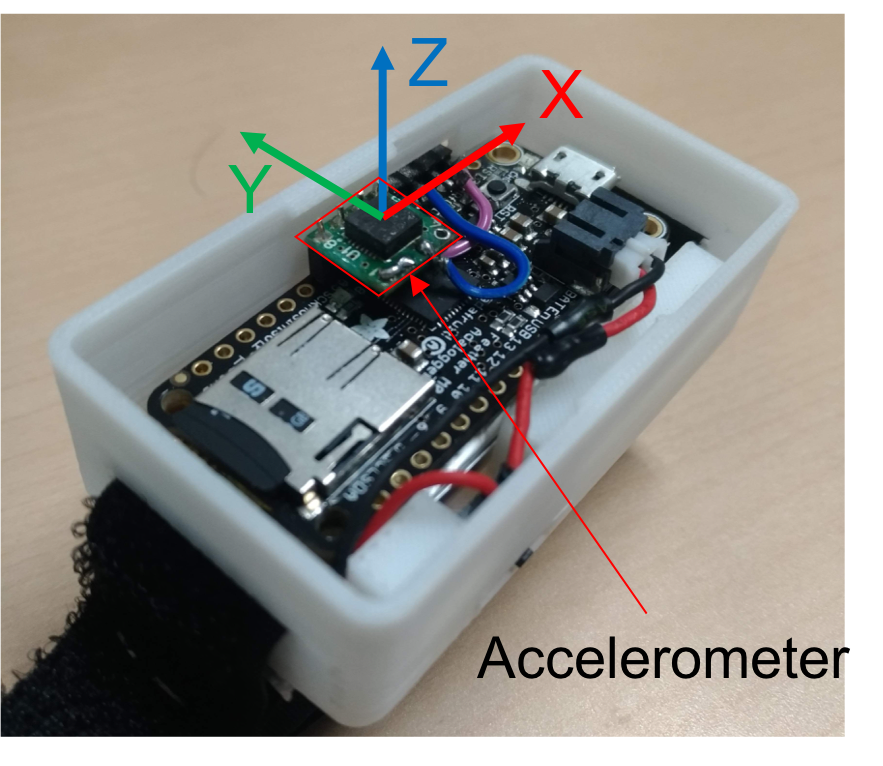
\includegraphics[width=0.5\linewidth]{fig/accelerometer_1}
  \caption{Accelerometer}
  \label{fig:accelerometer}
\end{figure}

\subsection*{データ記録部}
\subsubsection*{Arduino}
データ記録のため,マイクロコンピュータ基盤(Adafruit Faether M0 Adalogger)\cite{Utc2018}と32GBのSDcardを使用する.本デバイスで使用するマイクロコンピュータ基盤であるAdafruit Feather M0 Adaloggerは、Adafruit社製の小型Arduino互換ボードである.3.3Vで動作するプロセッサにはATSAMD21G18 ARM Cortex M0プロセッサを搭載している.
また,RAMには256KBのフラッシュメモリを搭載している.
寸法が51 x 23 x 8 mmと小さく,軽いためウェアラブルデバイス作成に適している.また,USBインターフェース、リチウムポリマー電池用のJST PH型2ピンコネクタを標準搭載しており,リチウムポリマー電池での駆動と充電が可能であるため本マイクロコンピュータ基盤を選定した.

\begin{figure}[H]
  \centering
  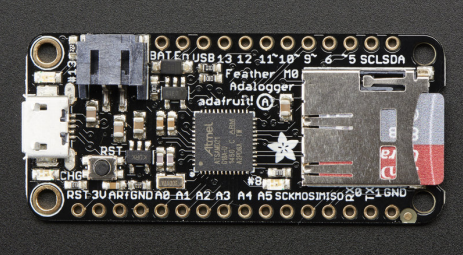
\includegraphics[width=0.5\linewidth]{fig/adafruit}
  \caption{Adafruit Faether M0 Adalogger\cite{Utc2018}}
  \label{fig:adafruit}
\end{figure}

\subsubsection*{Micro SD card}
赤外線距離センサと加速度センサからの信号は,信号の入力時間とともにマイコン基盤に接続されたMicro sdカードへ保存される.コンピュータへUSB2.0 A Male Microケーブルで接続することで,Micro sdカードに記録されたデータの転送が可能である.また,Micro SDcardは8GBのストレージ容量があり(最大で32GBに増設可能)
,365日以上分のデータの保存が可能である.


\begin{figure}[H]
  \centering
  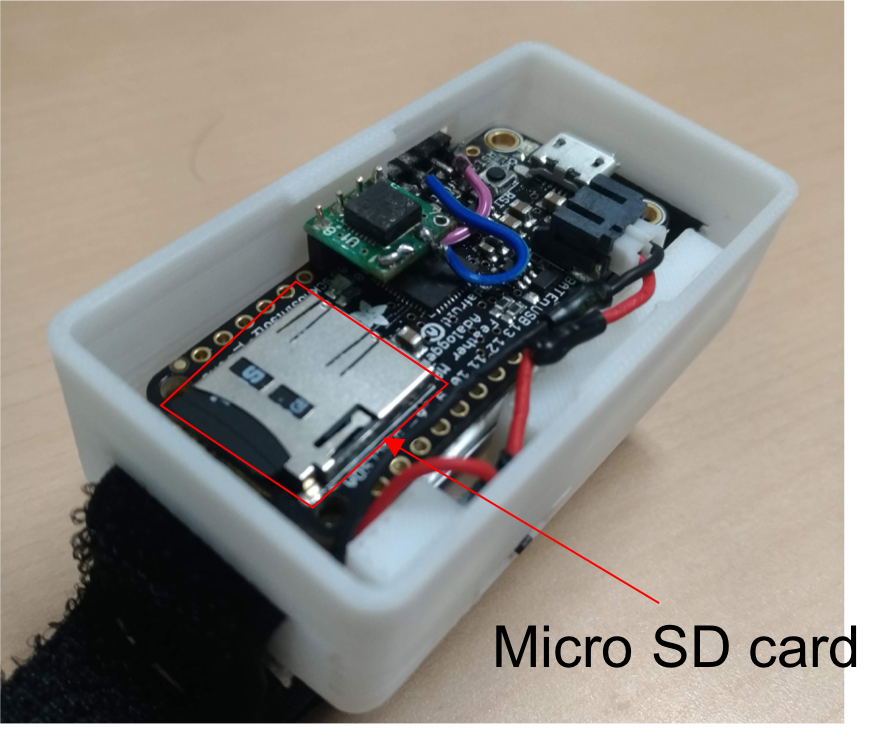
\includegraphics[width=0.5\linewidth]{fig/microsdcard}
  \caption{Micro SDcard}
  \label{fig:sd card}
\end{figure}


\subsubsection*{LiPo battery}
デバイスの電源として3.7V,400mAhのリポバッテリーを利用した.このバッテリーより24時間以上の連続電源供給が可能である.また,ウェアラブルデバイスと
コンピュータまたは,ACアダプターをUSB2.0 A Male Microケーブルで繋ぐことで,LiPo batteryの充電が可能である.LiPo batteryは30分でフル充電が可能である.
\begin{figure}[H]
  \centering
  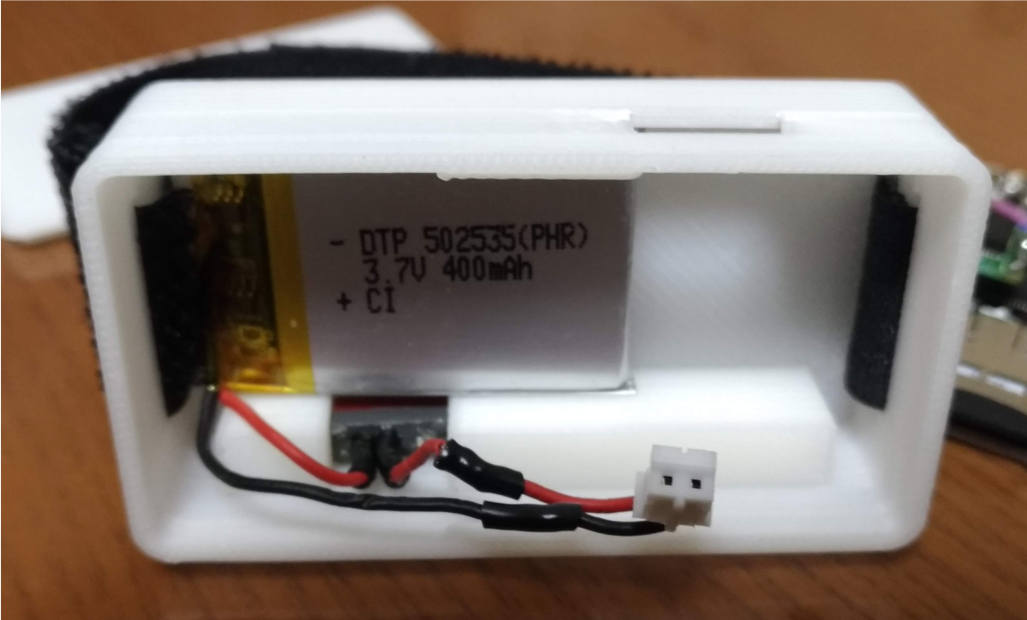
\includegraphics[width=0.5\linewidth]{fig/battery}
  \caption{A LiPo battery}
  \label{fig:battery}
\end{figure}

\begin{figure}[H]
  \centering
  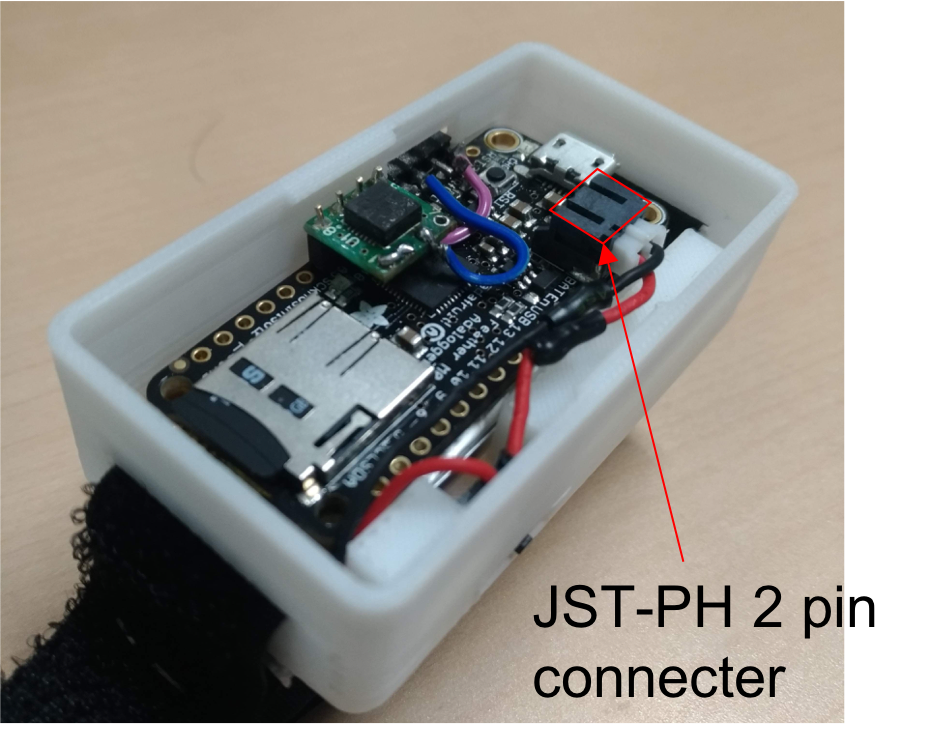
\includegraphics[width=0.5\linewidth]{fig/ph}
  \caption{connecter}
  \label{fig:connecter}
\end{figure}

\section{ピン配置}
Adafruits Feather M0 adaloggerはアナログ入力ピンが6チャンネルあり,10ビットのA/D変換が可能である.そのため,0-3.3Vの入力電圧を0-1023の整数値に変換することが可能である.これにより,単位当たり0.0032V(3.2 mV)の分解能を持つ.

赤外線距離センサをAdafruit Feather M0 adaloggerへ接続する際のピンヘッダを以下の表\ref{table:pin}に示す.
Adafruit Feather M0 adaloggerの3v3とGNDピンは電源供給を行うため,
Adafruit Feather M0 adaloggerのA0ピンはアナログピンであり,赤外線距離センサの電圧値を読み取る.
Adafruit Feather M0 adaloggerのA2ピンはアナログピンであり,加速度センサの電圧値を読み取る.

\begin{table}[H]
  \caption{Pin Installation}
  \centering
  \begin{tabular}{ccc}
    \hline
    Adafruit Feather M0 adalogger Pin & Infrared Distance Sensor Pin & Accelermeter Sensor Pin\\
    \hline \hline
    3v3 & Vcc & Vcc  \\
    GND & GND & GND  \\
    A0  & Vout& - \\
    A2  & -& Vout \\
    \hline
  \end{tabular}
   \label{table:pin}
\end{table}

\begin{figure}[H]
  \centering
  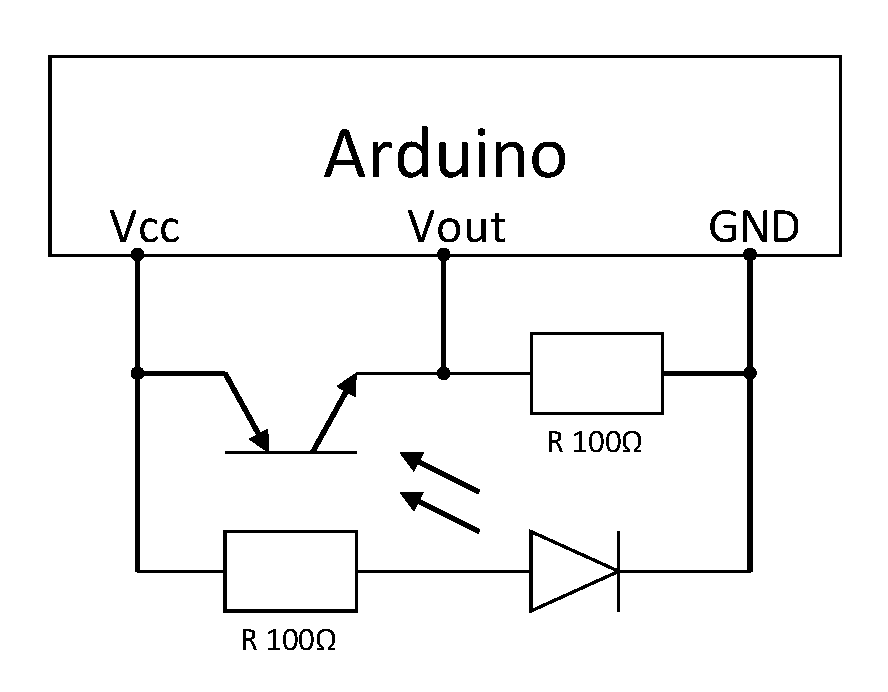
\includegraphics[width=0.5\linewidth]{fig/test}
  \caption{Circuit of Infrared distance sensor }
  \label{fig:circuit}{}
\end{figure}


\section{ファームウェアデザイン}
ファームウェアはArduinoボード,Adaruits Feather M0をArduino言語でプログラムした.電源を入れると,ファームウェアはArduinoボードがUSBによってコンピュータと接続しているか,確認する.USBで接続されている場合,自動でLiPo batteryの充電を行う.

\begin{figure}[H]
  \centering
  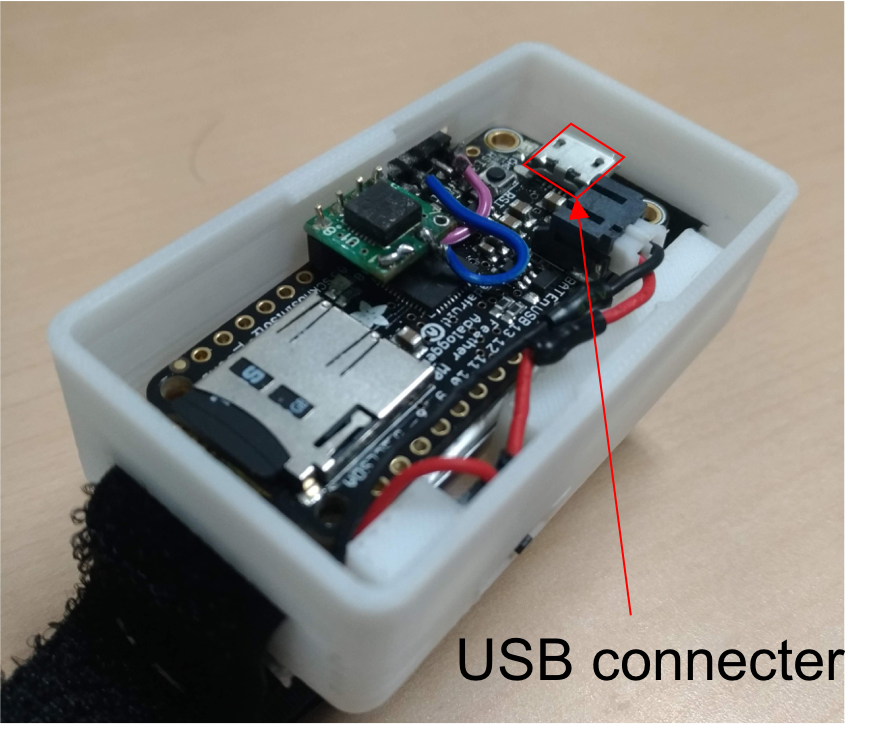
\includegraphics[width=0.5\linewidth]{fig/usbconne}
  \caption{USB connecter}
  \label{fig:USB connecter}
\end{figure}


USB接続がない場合は,データロガーモードに入る.microSDカードへの記録装置が有効になり,新しいcsvファイルが作成される.新しく作成されたcsvファイルには,三軸加速度センサと赤外線距離センサのセンシング情報と,電源がオンになってからの時間が記録される.つまり,csvファイルのカラムは加速度X,Y,Z軸それぞれ三つと,赤外線距離センサの一つ,さらにそれらのタイムスタンプを加えた五つのカラムである.三軸加速度センサと赤外線距離センサはともに10ビットの分解能で加速度,距離を検知するようプログラムされている.また,センシングのサンプリングレートは100Hzでプログラムされている.

\subsection{ウェアラブルデバイスの使用法}
\subsubsection*{コネクタの接続方法}
本デバイスは,赤外線距離センサが取り付けられた,指輪型ハードウェアと
加速度センサが搭載されたデータ記録部の腕輪型ハードウェアに分けられている.
腕輪型ハードウェアは,単体でも利用でき,加速度センサによるセンシングが可能である.
赤外線距離センサを利用するためには二つのハードウェアをコネクタで接続する必要がある.
コネクタをFig.\ref{fig:connecter}に示す.
本デバイスのコネクタはQI(2550)コネクタである.
腕輪型ハードウェアから出ているオス側のコネクタを,指輪型ハードウェアのメス型コネクタへ接続して使用する.
\begin{figure}[H]
  \centering
  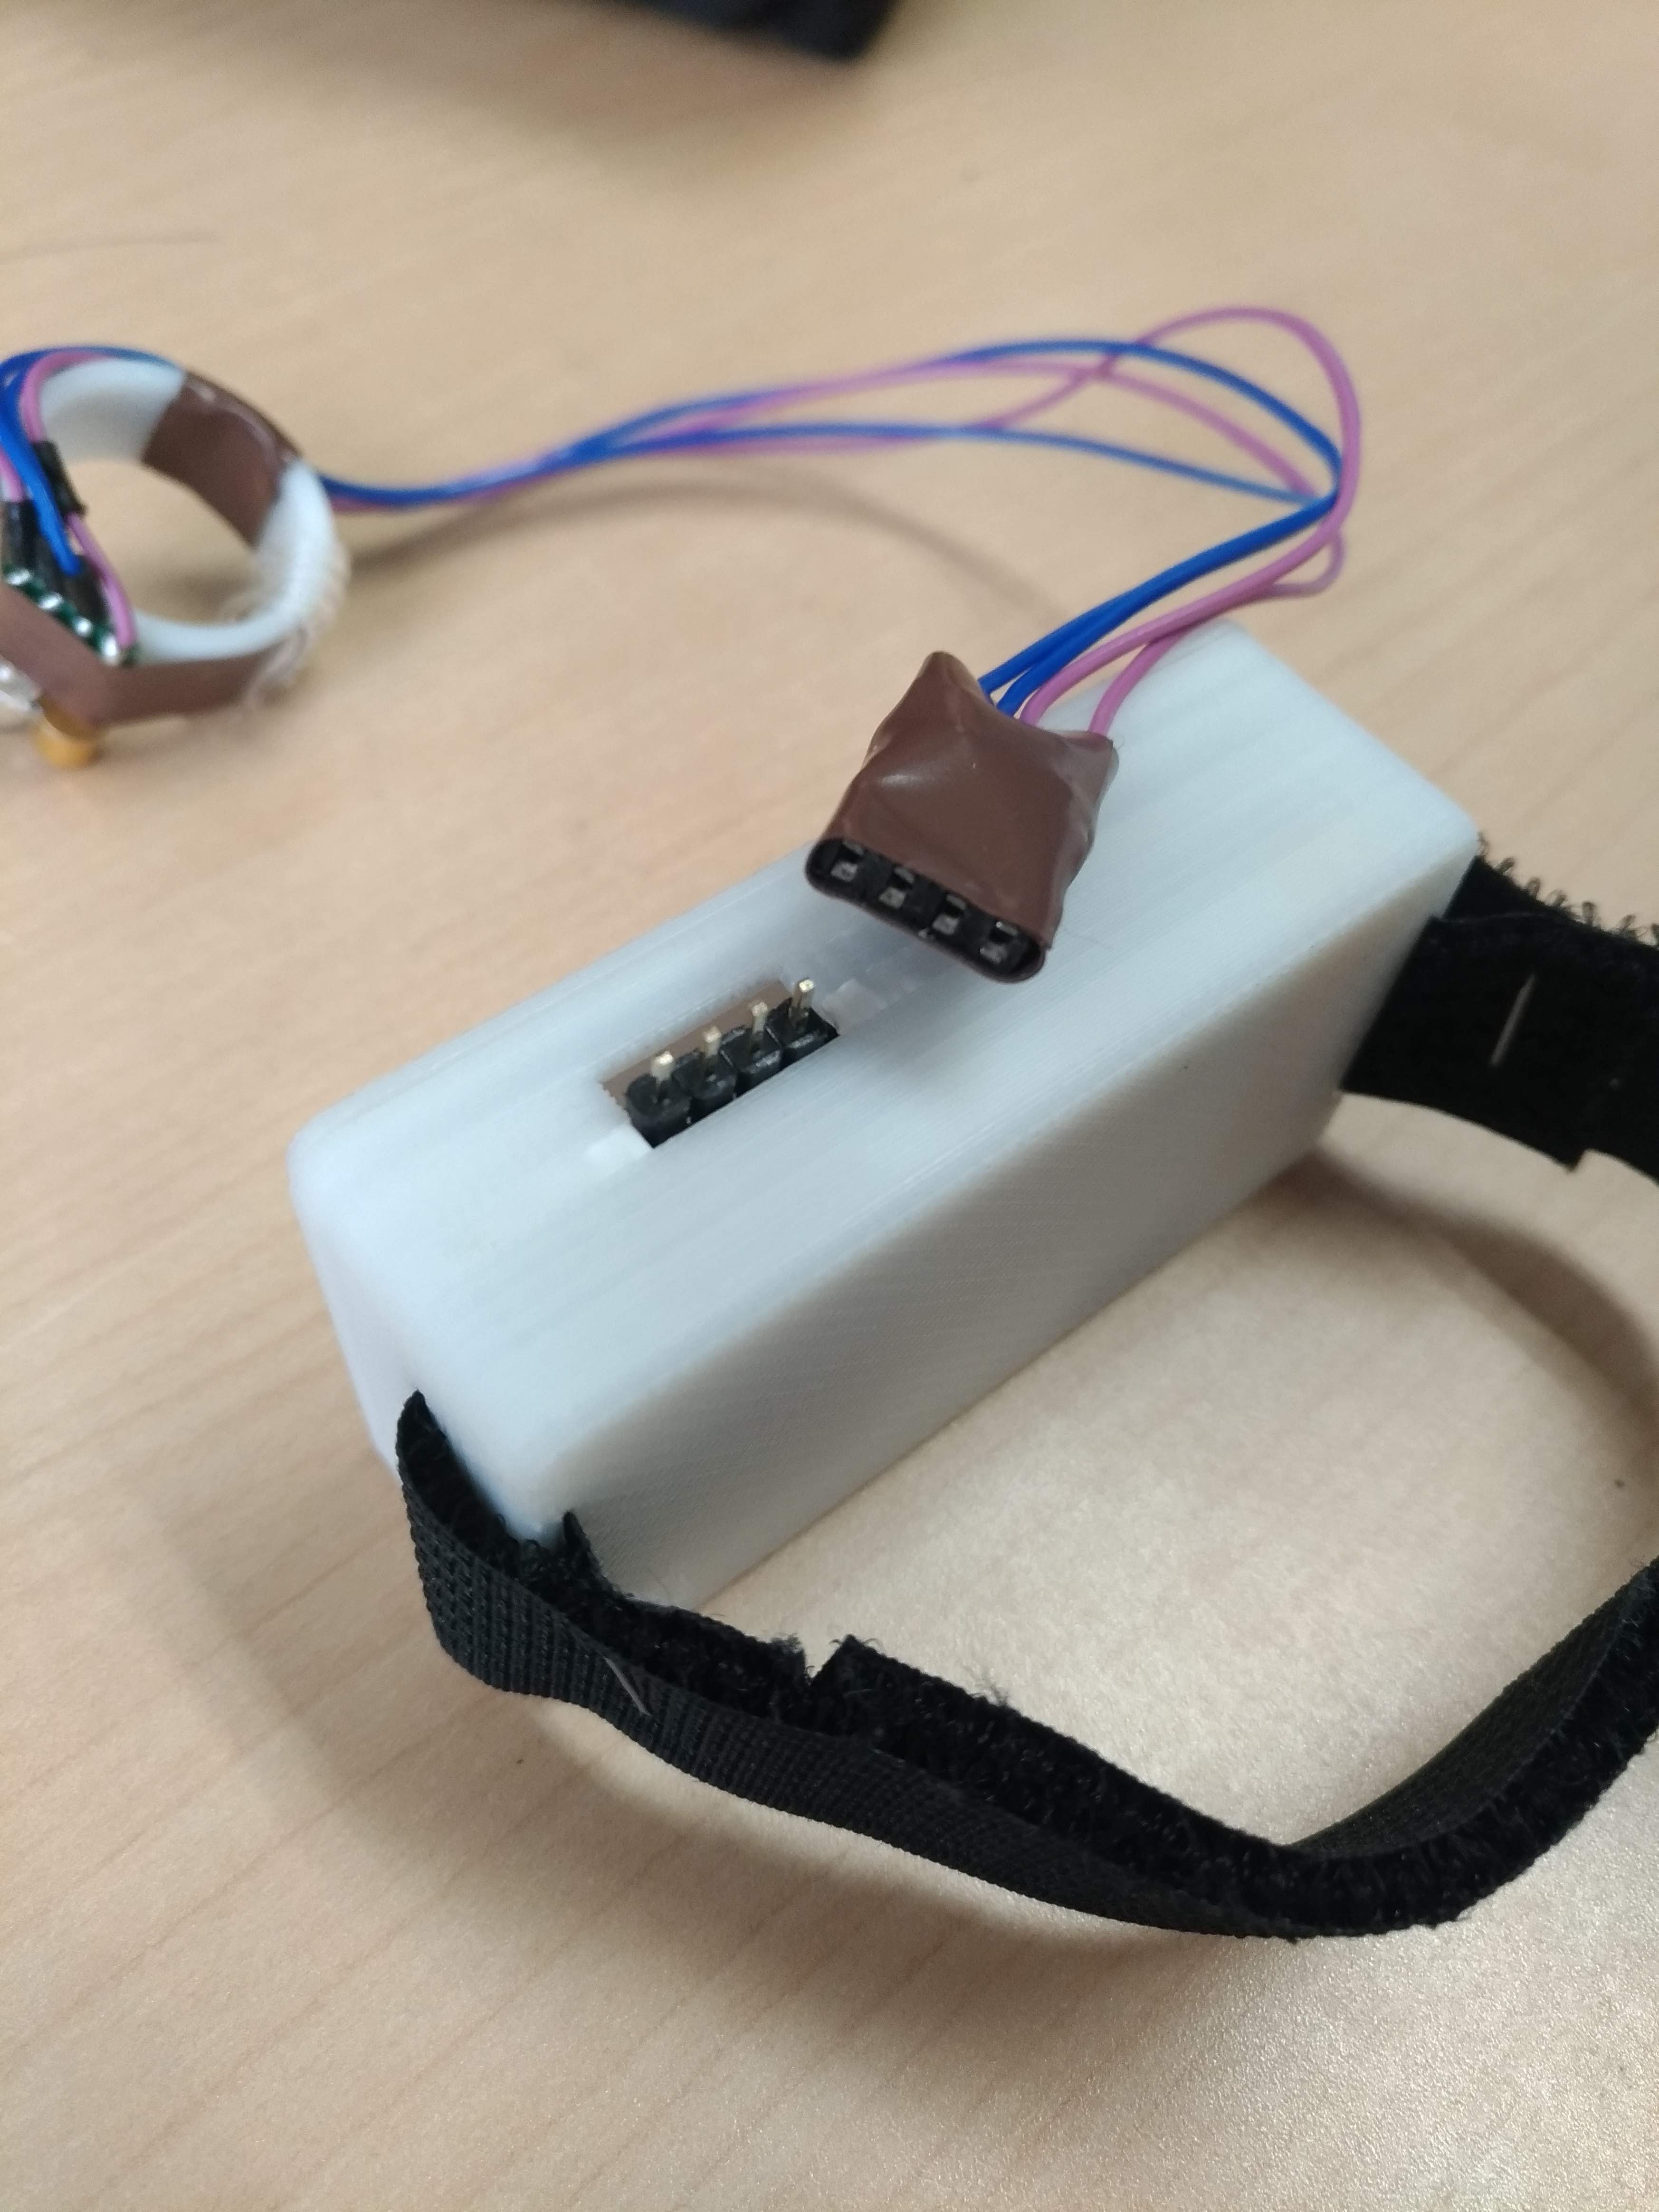
\includegraphics[width=0.5\linewidth]{fig/connecter.jpg}
  \caption{QI connecter}
  \label{fig:QI connecter}
\end{figure}


\subsubsection*{本デバイスの装着方法}
本デバイスの装着方法をFig\ref{fig:ring}に示す.指輪型のセンシング部は,食指の第二関節に装着し,ストレージ部は手首にマジックテープを使用し取り付ける.この際,指輪の大きさは,ユーザに合わせたものを選ぶ.また,赤外線距離センサ部が\ref{fig:principle}に示すように,手掌側になるよう装着する.
\begin{figure}[H]
  \centering
  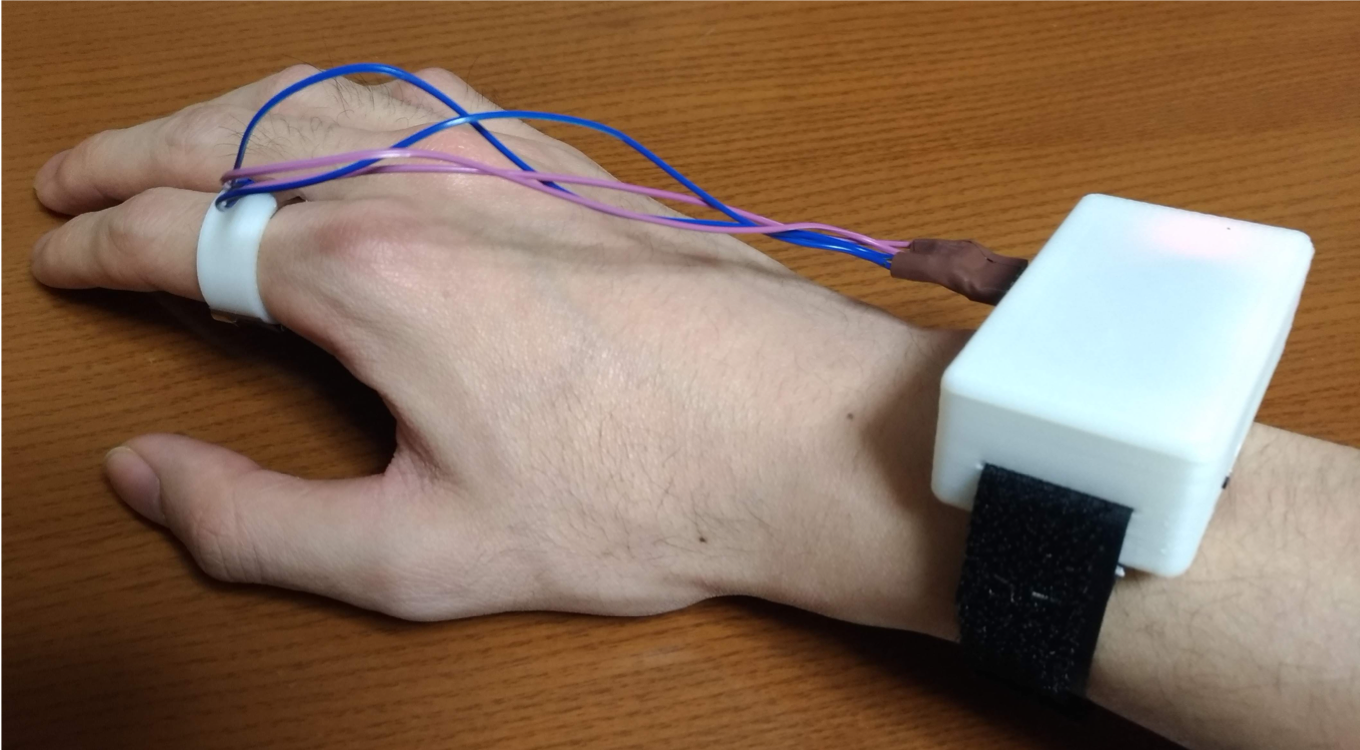
\includegraphics[width=0.8\linewidth]{fig/fal4.png}
  \caption{Ring worn on the index finger and Strage worn on the wrist}
  \label{fig:ring}
\end{figure}

\subsubsection*{電源の入れ方とデータ記録}
本デバイスに取り付けられたスイッチをスライドし電源をオンにした時より,赤外線距離センサと加速度センサのセンサ値の記録を開始する.
また,センサ値は,スイッチをオフにするまで連続計測,記録される.
各センサのセンサ値と,センサ値が計測された時間を保持するデータはCSVファイルでSD card内に保存される.
本デバイスに記録されたデータは,コンピュータと本デバイスをUSBケーブルで直接繋ぐか,Micro SDcardをコンピュータに移すことで,アクセスが可能である.

%スイッチの写真


\section{センシングキャリブレーション}
\subsection*{赤外線距離センサのキャリブレーション}
赤外線距離センサは物体に反射し,フォトトランジスタで受光した赤外線の強度を計測することで,距離を推定する.
しかし,同じ距離であっても赤外線が反射する物体によっては,違う
受光量となる場合がありえる.これは物体によって光の反射率が違い,同じ距離で計測したとしても,フォトトランジスタで受け取る受光量が違ってくるためである.つまり,人によって,指の長さや皮膚の色が違うため,同じセンサ値であっても,本来の距離が変わる問題がある.この問題を解決するために,被験者ごとに皮膚の反射率を調べることが望ましいが,本システムは日常生活での使用を目的としており,キャリブレーションがユーザに負荷をかけないことが求められる.
そのため,本システムでは計測される距離と受光量の関係を求め,キャリブレーションが可能な方法を提案する.キャリブレーションには以下の3つのパラメータを用いる.
\if0
\begin{itemize}
 \item デバイスを装着する指の長さ
 \item 指伸展時のセンサ情報
 \item 指屈曲時のセンサ情報
\end{itemize}
\fi

\begin{table}[H]
  \caption{赤外線距離センサのキャリブレーションに必要なパラメータと計測方法}
  \label{table:cali_inf}
  \centering
  \begin{tabular}{ll}
    \hline
    Parameter &  Measurement  \\
    \hline \hline
デバイスを装着する指の長さ&
デバイスを装着している指の,第二関節から指先までの長さをメジャーにより計測\\

指伸展時のセンサ情報&
指の伸展を3秒間保持し,その間,デバイスの電源を入れ赤外線距離センサで計測\\

指屈曲時のセンサ情報&
指の屈曲を3秒間保持し,その間,デバイスの電源を入れ赤外線距離センサで計測\\

    \hline
  \end{tabular}
\end{table}

デバイスを装着する指の長さは,第二関節から指先までの長さをメジャーを用い,計測した.計測で得られた第二関節から指先までの長さのデータについては後に記述する.指伸展時のセンサ情報と指屈曲時のセンサ情報については,ユーザに指輪型センシング部を装着し,ユーザに指を伸展または屈曲し,3秒間保持してもらう.指姿勢保持中に赤外線距離センサの計測を行い3秒間センシングする.このとき得られたセンサ値をそれぞれ,指伸展時のセンサ情報と指屈曲時のセンサ情報とした.得られたセンサ情報と指の長さのデータにより,線形近似を行い,ユーザごとのキャリブレーションを行った.Fig.\ref{fig:cali_inf}は指の伸展時のセンサ情報が0.2V,屈曲時のセンサ情報が1.05V,第二関節から指先までの長さが5cmのユーザのキャリブレーションを行った時の線形近似モデルである.この方法により,ユーザの肌の色が異なることによる,反射物の反射率の違いや,ユーザの指の長さによる計測誤差のキャリブレーションが可能である.

\begin{figure}[H]
  \centering
  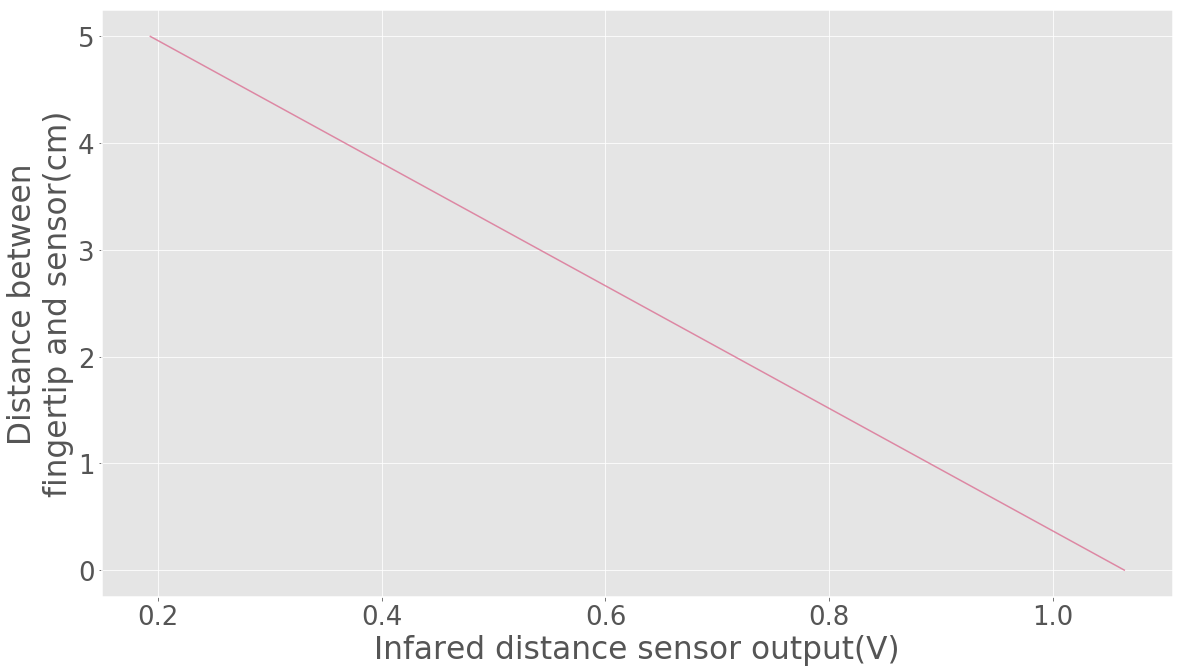
\includegraphics[width=0.8\linewidth]{fig/infrared_linearmodel}
  \caption{Infrared distance sensor linear model }
  \label{fig:cali_inf} 
\end{figure}

\subsection*{加速度センサのキャリブレーション}
加速度センサはユーザごとにキャリブレーションをする必要がない.しかし,センサからマイクロコンピュータボードへ出力されるのは電圧値であるため,電圧値を加速度へ変換する必要がある.加速度センサのキャリブレーションは,重力加速度が$9.8m/s^2$であることを利用し行なった.加速度センサの各軸ごとに
平面と平行になるようセンサの向きを合わせ,平面にデバイスを置いた状態で3秒間電源をオンにし,センサ情報を記録した.さらに,加速度センサの各軸ごとにセンサの向きを,先ほどの記録時とは反対向きにした.その後,センサから3秒間出力された電圧値を平均し,重力加速度の$9.8m/s^2$を用いて,線形近似Fig.\ref{fig:cali_accel}し,電圧値から加速度への変換を行なった.この操作を,加速度センサの各軸に行い,キャリブレーションをした.

重力加速度$9.8m/s^2$がかかっている時の,センサ値を,加速度センサの各軸において記録し,線形モデルを作成した.

\begin{figure}[H]
  \centering
  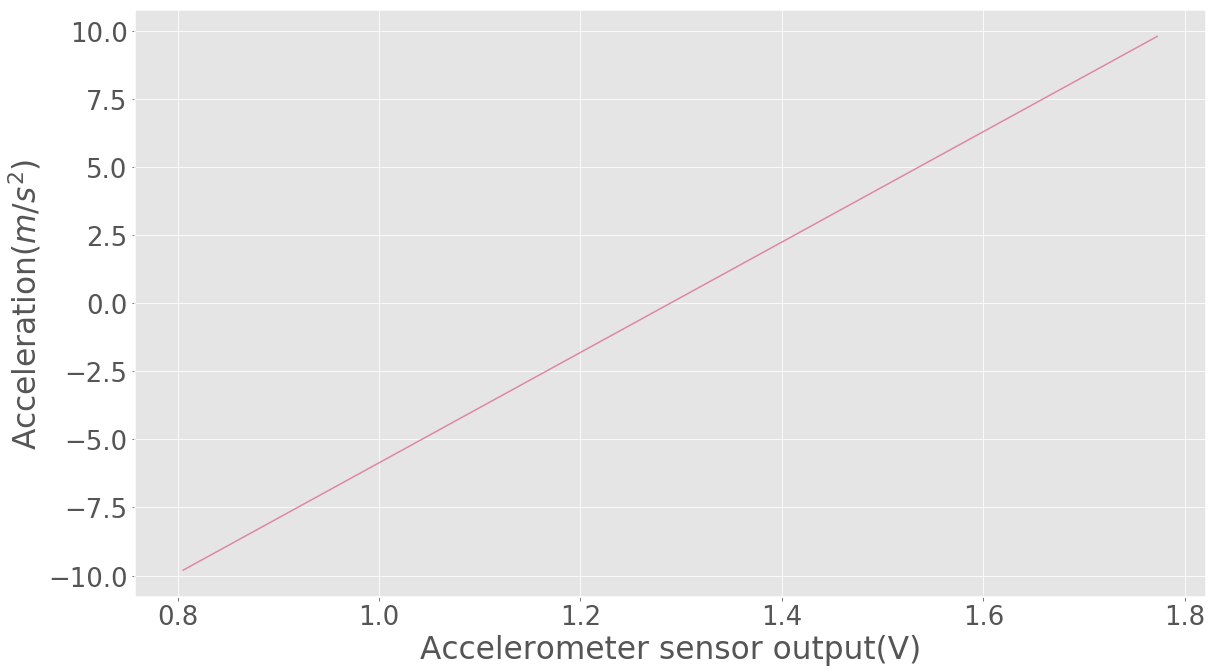
\includegraphics[width=0.8\linewidth]{fig/accel_linearmodel}
  \caption{Accelerometer sensor linear model }
  \label{fig:cali_accel}
\end{figure}

\section{センシング情報の処理方法}
アナログセンサの電圧値は$2^{10}$の分解能を持つデジタル信号に変換される.
センサ情報の前処理として,複数の処理を行った.
まず始めに,センシング情報の補完を行なった.
センシングのサンプルレートは100Hzであるが,Arduinoにより得られる赤外線距離センサと加速度センサ情報のタイムスタンプは正確に,0.01秒刻みで得ることができない.なぜならば,センサ情報の取得にはArduino内部のプログラムを用いており,センサ情報を取得するために,0.01秒ごとにプログラムをループしているため,プログラムの実行時間にずれが生じるからである.また,本実験で用いている,Arduinoボード(Adafruits Feather M0)は48MHz動作のArduinoボードであり,このArduinoの時間分解能は12マイクロ秒であることも理由の一つである.
よって,得られたセンシング情報を線形補完し,100Hzのセンシング情報に変換した.
次に,デバイスにより取得できるセンシングデータは,環境ノイズを含んでいるため,ノイズの除去を行った.
ノイズの除去はバターワイスローパスフィルターにより,25Hz以上の周波数を持つシグナルをカットオフした.
カットオフする周波数は人の最も速い動作の周波数である25Hz\cite{Friedman2014,VanGalen1990,Mason2001,Simone2007}に設定した.
次に,キャリブレーション時に求めた,線形近似モデルにより,加速度センサ,赤外線距離センサから得られた電圧値をそれぞれ,加速度,距離に変換する.



赤外線距離センサのセンシングデータから指間接角度を推定する際、いくつかの信号処理を行った.さらに、指の使用量へ変換する処理も行った.それら処理を以下に示す.

\begin{enumerate}
 \item 線形補間により,センシングデータを100Hzのデータに変換した.
 \item 100Hzのサンプリングレートをもつセンシングデータに対し25Hzのローパスフィルタをかけノイズを除去した.
 \item 関節角度が90度,0度のときのセンシングデータを利用し,キャリブレーションを行った.
 \item 1次元線形回帰により、センシングデータを,センサから指までの距離へ変換した.
 \item 光の強さが光源からの距離の2乗に反比例する(逆二乗の法則)ため,距離データの補正を行なった.
 \item 式\ref{eq:theta}により,距離を角度に変換した.
 \item 角度を時間微分し,0.01秒間の変化角度(角速度)を導出した.
 \item 加速度を時間微分し,0.01秒間の加加速度(躍度)を導出した.
 \item 導出した角速度の絶対値を導出した.
 \item xyz軸の躍度のノルムをとった.
 \item タスクごとに,角速度,躍度を合計し,使用量を導出した.
\end{enumerate}


以下に,関節角度のデータから指の使用量を導出する,データ処理方法を記述する.
\begin{table}[H]
  \caption{Tasks}
  \label{table:tasks}
  \centering
  \begin{tabular}{ll}
    \hline
    Task &  Detail  \\
    \hline \hline
箸を使い食事&
被験者は利き手に箸を持ち,三つの皿に分けられた食品を口に運び食す.\\

布巾でテーブルを拭く&
被験者は利き手に布巾を持ち,70cm四方のテーブルを拭く.\\

タイピング&
被験者は両手を用い,タイピングゲームを行う.\\

ライティング&
被験者は利き手にボールペンを持ち,文字の書き取りを行う.\\

布巾を畳む&
被験者は両手を用い,布巾を四つ折りに畳む,広げるを繰り返す.\\

Hole peg testを行う&
被験者は利き手で十本のペグをホールに入れ,全てのペグをホールから抜き出す.\\

    \hline
  \end{tabular}
\end{table}


Fig.\ref{fig:angle}は,被験者がTable\ref{table:tasks}のタスクを表の上のタスクから,各5分ごと行った時の,関節角度のデータのプロットである.

\begin{figure}[H]
  \centering
  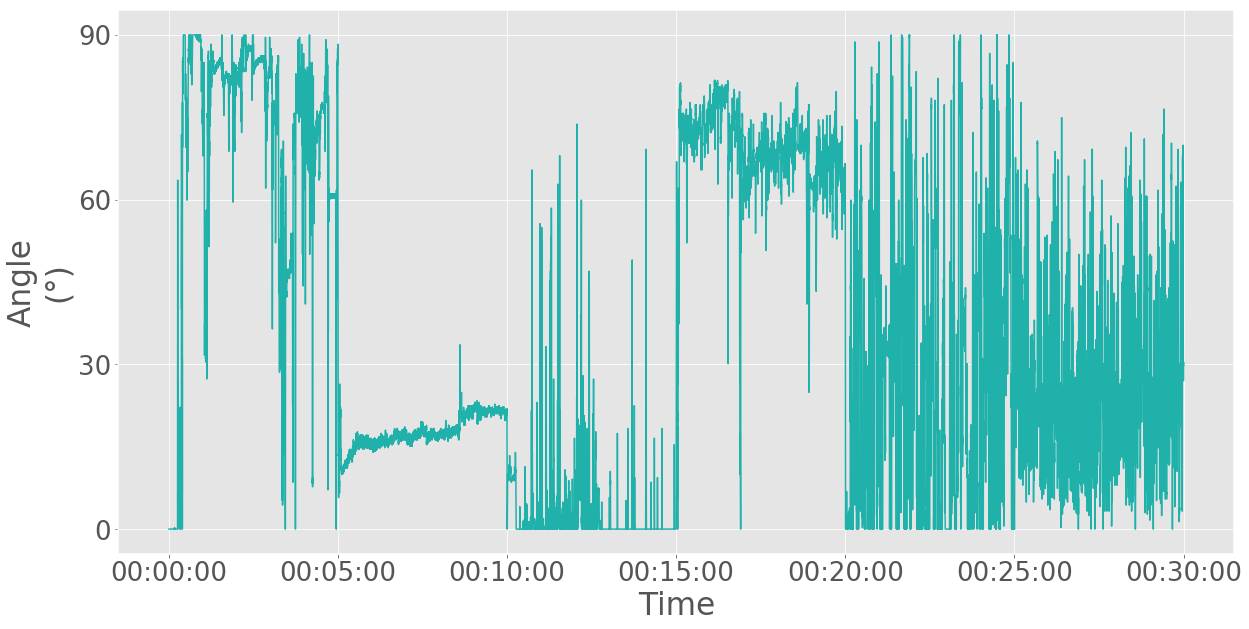
\includegraphics[width=0.8\linewidth]{fig/angle_}
  \caption{Data processing angle}
  \label{fig:angle}
\end{figure}

関節角度$\theta_i$から,0.01秒ごとの関節角度の変化量である角速度$\omega_i$を求める.
\begin{eqnarray}
\omega_i & = \theta_i /dt
\end{eqnarray}

\begin{figure}[H]
  \centering
  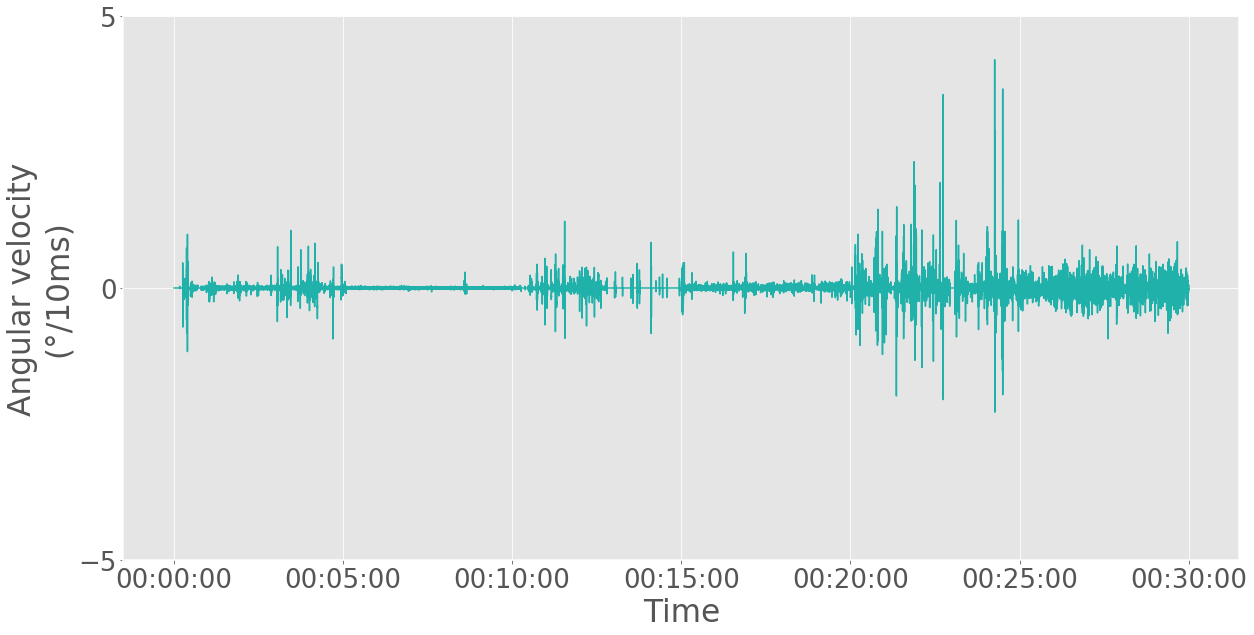
\includegraphics[width=0.8\linewidth]{fig/velocity}
  \caption{Data processing angle velocity}
  \label{fig:angle_velocity}
\end{figure}

その後,角速度$\omega_i$の絶対値を導出する.

\begin{figure}[H]
  \centering
  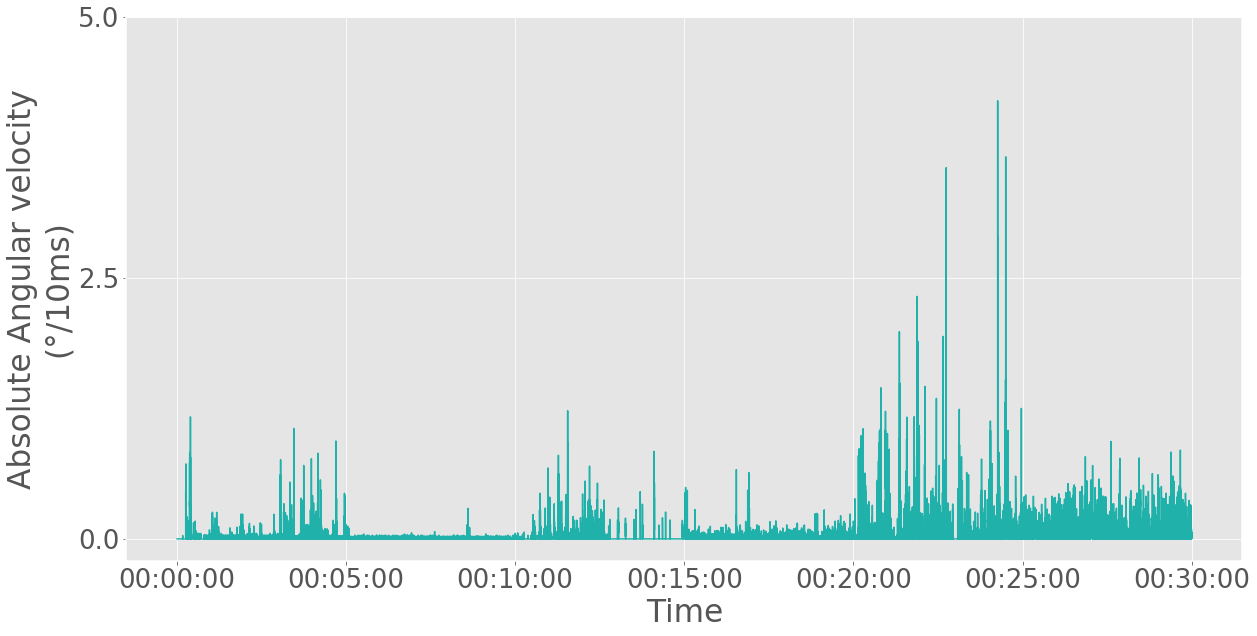
\includegraphics[width=0.8\linewidth]{fig/absolute_velocity}
  \caption{Data processing absolute angle velocity}
  \label{fig:abs_velocity}
\end{figure}

5分間のタスクごとに,関節角度の変化量の合計を導出する.
\begin{eqnarray}
Aggrigated\ angle  = \sum_{i=1}^n |\omega_i|
\end{eqnarray}

ここで,nはタスクごとのサンプル数であるため,300秒$\times$100Hzより,
$n=30000$である.
\ref{fig:agg_angle}は5分間のタスクごとに,関節角度の変化量の合計を示したグラフである.


\begin{figure}[H]
  \centering
  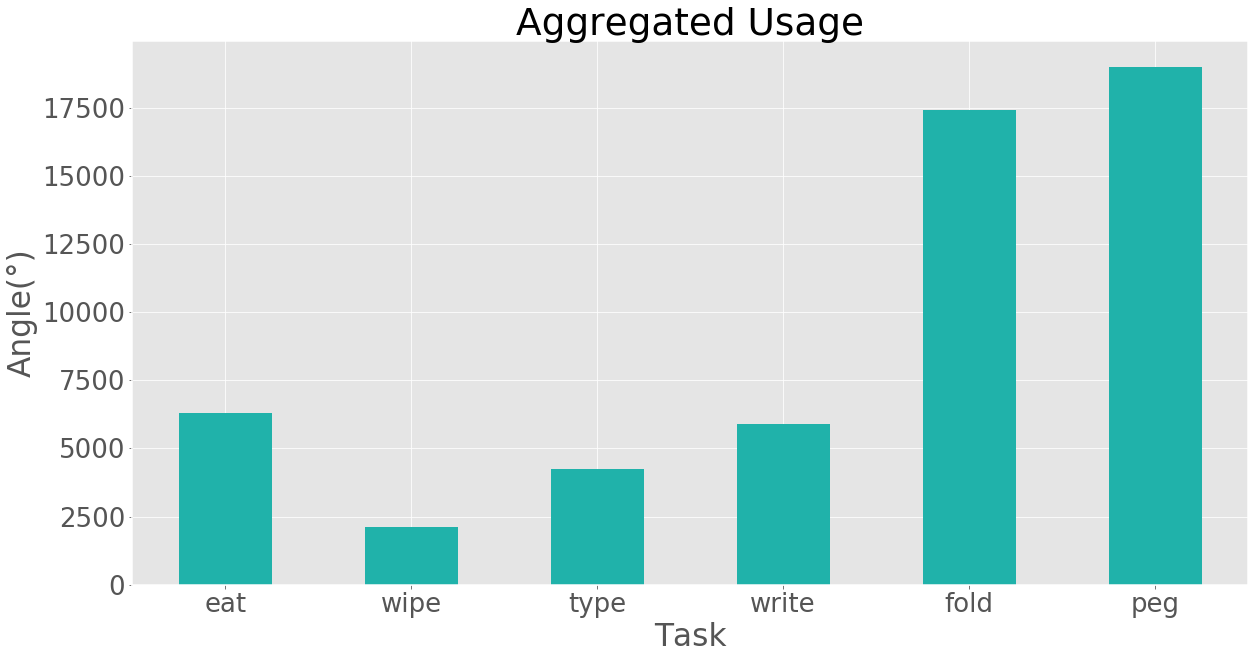
\includegraphics[width=0.8\linewidth]{fig/aggrigated_angle}
  \caption{Data processing aggrigated angle}
  \label{fig:agg_angle}
\end{figure}



以下に,加速度のデータから腕の使用量を導出する,データ処理方法を記述する.
Fig.\ref{fig:accel_xyz}は,被験者がTable\ref{table:tasks}のタスクを表の上のタスクから,
各5分ごと行った時の,加速度データのプロットである.

\begin{figure}[H]
  \centering
  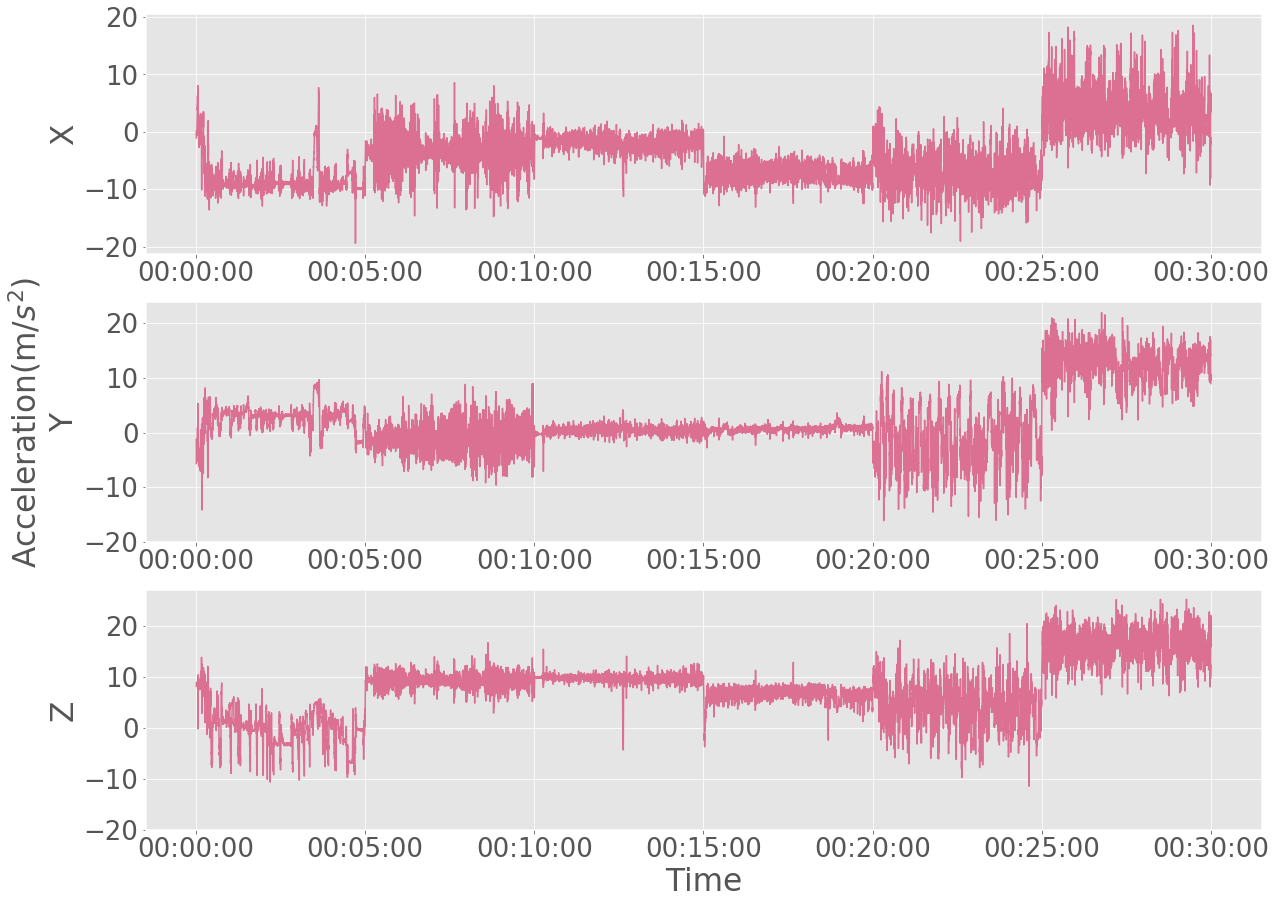
\includegraphics[width=0.8\linewidth]{fig/accel_xyz}
  \caption{Data processing acceleration}
  \label{fig:accel_xyz}
\end{figure}


それぞれの軸の躍度は以下の式\ref{eq:jerkxyz}で表される.

\begin{eqnarray}
j_x & = da_x/dt\\
j_y & = da_y/dt\\
j_z & = da_z/dt
\label{eq:jerkxyz}
\end{eqnarray}

$a_{x,i}, a_{y,i},a_{z,i}$をx,y,z軸の$i$秒の時の加速度とする.また,サンプリングレート100Hzより$dt=0.01$とする.
これらより,それぞれの軸の加速度から躍度を導出すると以下のFig.\ref{fig:jerk_xyz}が得られる.

\begin{figure}[H]
  \centering
  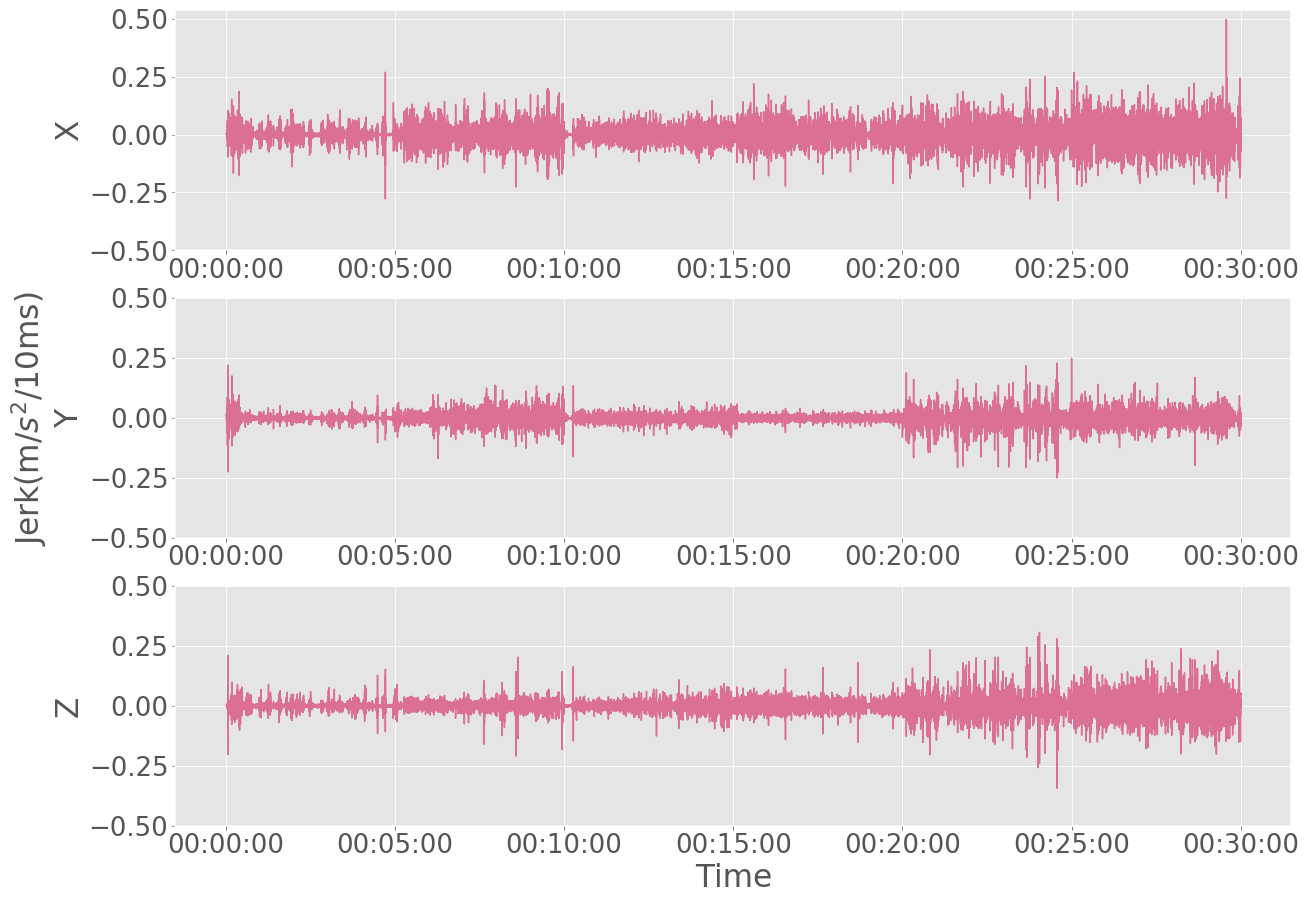
\includegraphics[width=0.8\linewidth]{fig/jerk_xyz}
  \caption{Data processing each axial jerk}
  \label{fig:jerk_xyz}
\end{figure}

それぞれの軸について得られた躍度のノルムを式\ref{eq:jerknorm}によって導出すると

\begin{equation}
j_{norm,i} = \sqrt{{j_{x,i}}^2+{j_{y,i}}^2+{j_{z,i}}^2}
\label{eq:jerknorm}
\end{equation}
であり,$j_{norm,i}$をプロットすると
以下のFig.\ref{fig:norm_jerk}が得られる.

\begin{figure}[H]
  \centering
  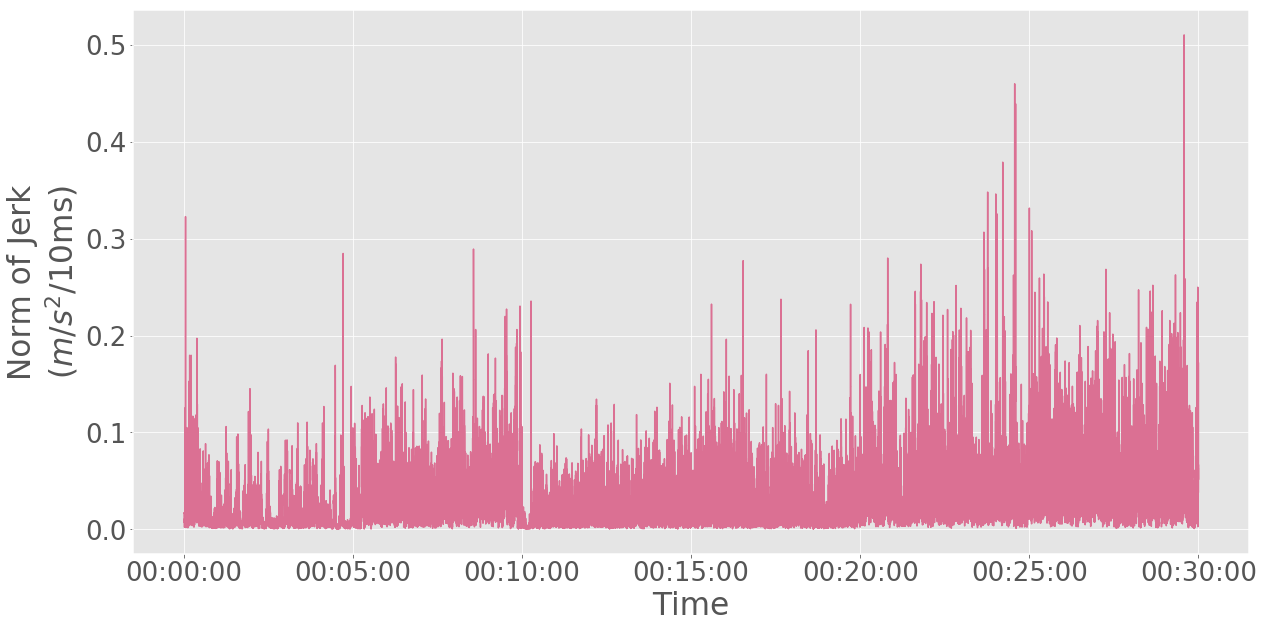
\includegraphics[width=0.8\linewidth]{fig/norm_jerk}
  \caption{Data processing norm of jerk}
  \label{fig:norm_jerk}
\end{figure}

5分間のタスクごとに,加速度の変化量の合計を導出する.
\begin{eqnarray}
Aggrigated\ accleration  = \sum_{i=1}^n j_{norm,i}
\end{eqnarray}

ここで,nはタスクごとのサンプル数であるため,300秒$\times$100Hzより,
$n=30000$である.
\ref{fig:agg_accel}は5分間のタスクごとに,加速度の合計を示したグラフである.

\begin{figure}[H]
  \centering
  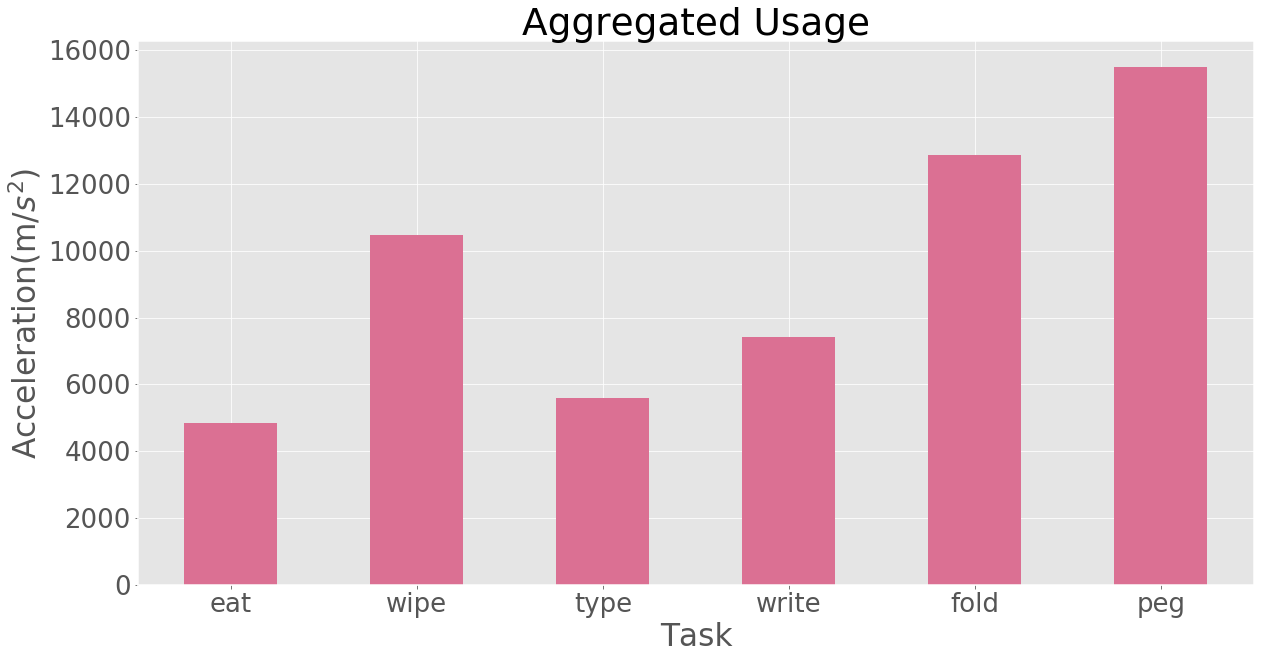
\includegraphics[width=0.8\linewidth]{fig/aggrigated_accel}
  \caption{Data processing aggrigated acceleration}
  \label{fig:agg_accel}
\end{figure}

